\begin{tikzpicture}[remember picture,overlay,
titlebox/.style = {text width = 10cm, font = \huge},
box/.style = {text width = 8cm, font = \LARGE}]
    %
    \draw($(current page.north west)+(1.75,-1.5)$) rectangle ++(11.3,-18);
    % Thesis title
    \node[anchor=west,titlebox] at ($(current page.north west)+(2.4,-6)$) {
        \begin{center}
            \textbf{{\Huge A} Semi-incremental Model Order Reduction Approach for Fatigue Damage Computations}
        \end{center}
    };
    %
    \node[anchor=west, box] at ($(current page.north west)+(3.4,-13.5)$) {
        \begin{center}
            %
            Von der\\
            %
            \vspace{0.5cm}
            %
            Fakult\"at f\"ur Bauingenieurwesen und Geod\"asie\\
            %
            der Gottfried Wilhelm Leibniz Universit\"at Hannover\\
            %
            zur Erlangung des Grades\\
            %
            \vspace{0.5cm}
            %
            \textit{Doktor-Ingenieur (Dr.-Ing.)}\\
            %
            \vspace{0.5cm}
            %
            genehmigte Dissertation
            %
            \vspace{1cm}
            %
            von\\
            %
            Shadi Alameddin, M.Sc.\\
            %
            \vspace{1cm}
            %
            Erscheinungsjahr 2020\\
            %
        \end{center}
    };
    
    %
    % Add yourself
    % \node[anchor=west] at (6.8,13.6) {\small\textbf{Doktorand:}};
    % \node[anchor=west] at (6.8,13.1) {\small\textit{D. Beurle}};
    
    % % Add secondary examiners
    % \node[anchor=west] at (6.8,14.25) {\small\textit{Prof. Dr. R. Desmorat}};
    % \node[anchor=west] at (6.8,14.7) {\small\textit{Prof. Dr.-Ing. M. Andr\'e}};
    % \node[anchor=west] at (6.8,15.2) {\small\textbf{Korreferenten:}};
    
    % Add main supervisor
    % \node [anchor=west] at (6.8,16.4) {\small\textbf{Hauptreferenz:}};
    % \node [anchor=west] at (6.8,15.9) {\small\textit{Prof. Dr.-Ing. U. Nackenhorst}\\};

\end{tikzpicture}
\newpage
\thispagestyle{empty}
\begin{tikzpicture}[remember picture,overlay,
box/.style = {text width = 5cm, font = \large}]
%
\draw($(current page.north west)+(1.75,-1.5)$) rectangle ++(11.3,-18);
%
\node[anchor=west,box](n1) at ($(current page.north west)+(1.8,-10.5)$) {
	%        
	\textbf{Referent:} \\
	Prof. Dr.-Ing. U. Nackenhorst
	%        
	\medskip
	
	\textbf{Korreferenten:}\\
	Prof. Dr. David N\'{e}ron
	%        
	\medskip
	
	\textbf{Tag der Promotion:}\\
	06. Februar 2020
	%
	\medskip
	
	\textbf{Herausgeber:}\\
	Prof. Dr.-Ing. U. Nackenhorst
	%        
	\bigskip
	\bigskip
	
	\textbf{Verwaltung:} \\
	Institut f\"ur Baumechanik und Numerische Mechanik \\
	Gottfried Wilhelm Leibniz Universit\"at Hannover\\
	Appelstr. 9A\\
	30167 Hannover\\
	Tel.: +49 (0)511 / 762-3560\\
	Fax.: +49 (0)511 / 762-19053\\
	%        
	\bigskip
	\bigskip
	
	Shadi Alameddin\\
	\medskip
	Institut f\"ur Baumechanik und Numerische Mechanik\\
	Gottfried Wilhelm Leibniz Universit\"at Hannover\\
	Appelstr. 9A\\
	30167 Hannover\\
	%        
	\bigskip
	\bigskip
	% License
	% Creative Commons BY 4.0 for open access
	
\includegraphics[width=0.8cm]{./z_ibnm/cc.eps}
	\includegraphics[width=0.8cm]{./z_ibnm/by.eps}
	%        
	Licensed under Creative Commons Attribution 4.0 International\\
	(CC BY 4.0).
	%
	% Hold all the rights
	% Alle Rechte, insbesondere das der
	% Ubersetzung in fremde Sprachen,
	% Vorbehalten. Ohne Genehmigung
	% des Autors ist es nicht gestattet,
	% dieses Heft ganz oder teilweise
	% auf photomechanischem, elektronischem oder
	% sonstigem Wege zu vervielf\"altigen
	%        
	\bigskip
	
	Typeset in FreeSerif with \LaTeX
	%        
	\bigskip
	
	ISBN 978-3-935732-51-2
};
\end{tikzpicture}